\documentclass[tikz, border=1mm]{standalone}
\usetikzlibrary{bayesnet}

\begin{document}
    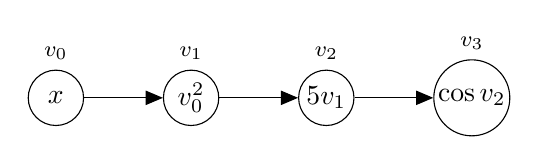
\begin{tikzpicture}
        % Define nodes
        % measurements
        \node[latent, label=above:{$v_0$}](v_0){$x$}; %
        \node[latent, right=of v_0,label=above:{$v_1$}](v_1){$v_0^2$}; %
        \node[latent,right=of v_1,label=above:{$v_2$}](v_2){$5v_1$}; %
        \node[latent,right=of v_2,label=above:{$v_3$}](v_3){$\cos v_2$}; %
        \edge {v_0} {v_1} ;
        \edge {v_1} {v_2} ;
        \edge {v_2} {v_3} ;       
    \end{tikzpicture}
\end{document}